\documentclass{beamer}

\usepackage{tikz}
\usepackage{graphiso}

\begin{document}

\begin{frame}
  \begin{center}
    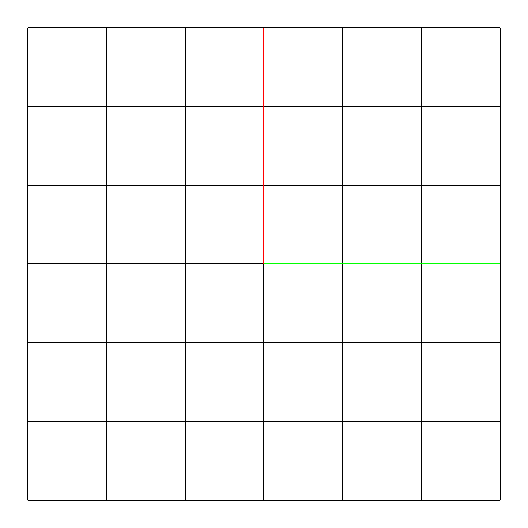
\begin{tikzpicture}
      \useasboundingbox (-3,-3) rectangle (3,3);
      \draw (-3,-3) grid (3,3);
      \draw[green] (0,0) -- (3,0);
      \draw[red] (0,0) -- (0,3);
      \VertexM[xa=-3,ya=3,xb=3,yb=2,shows=2,starts=3,stops=10]{x}
      \VertexM[xa=-3,ya=-3,xb=3,yb=-2,shows=2,starts=3,stops=10]{y}
      \only<2->{\Edge(x)(y)}
    \end{tikzpicture}
  \end{center}
\end{frame}

\end{document}
